\section{Referencia de la Clase familiasview}
\label{classfamiliasview}\index{familiasview@{familiasview}}
Muestra y administra la ventana de familias de art\'{\i}culos.  


{\tt \#include $<$familiasview.h$>$}

Diagrama de colaboraci\'{o}n para familiasview:\begin{figure}[H]
\begin{center}
\leavevmode
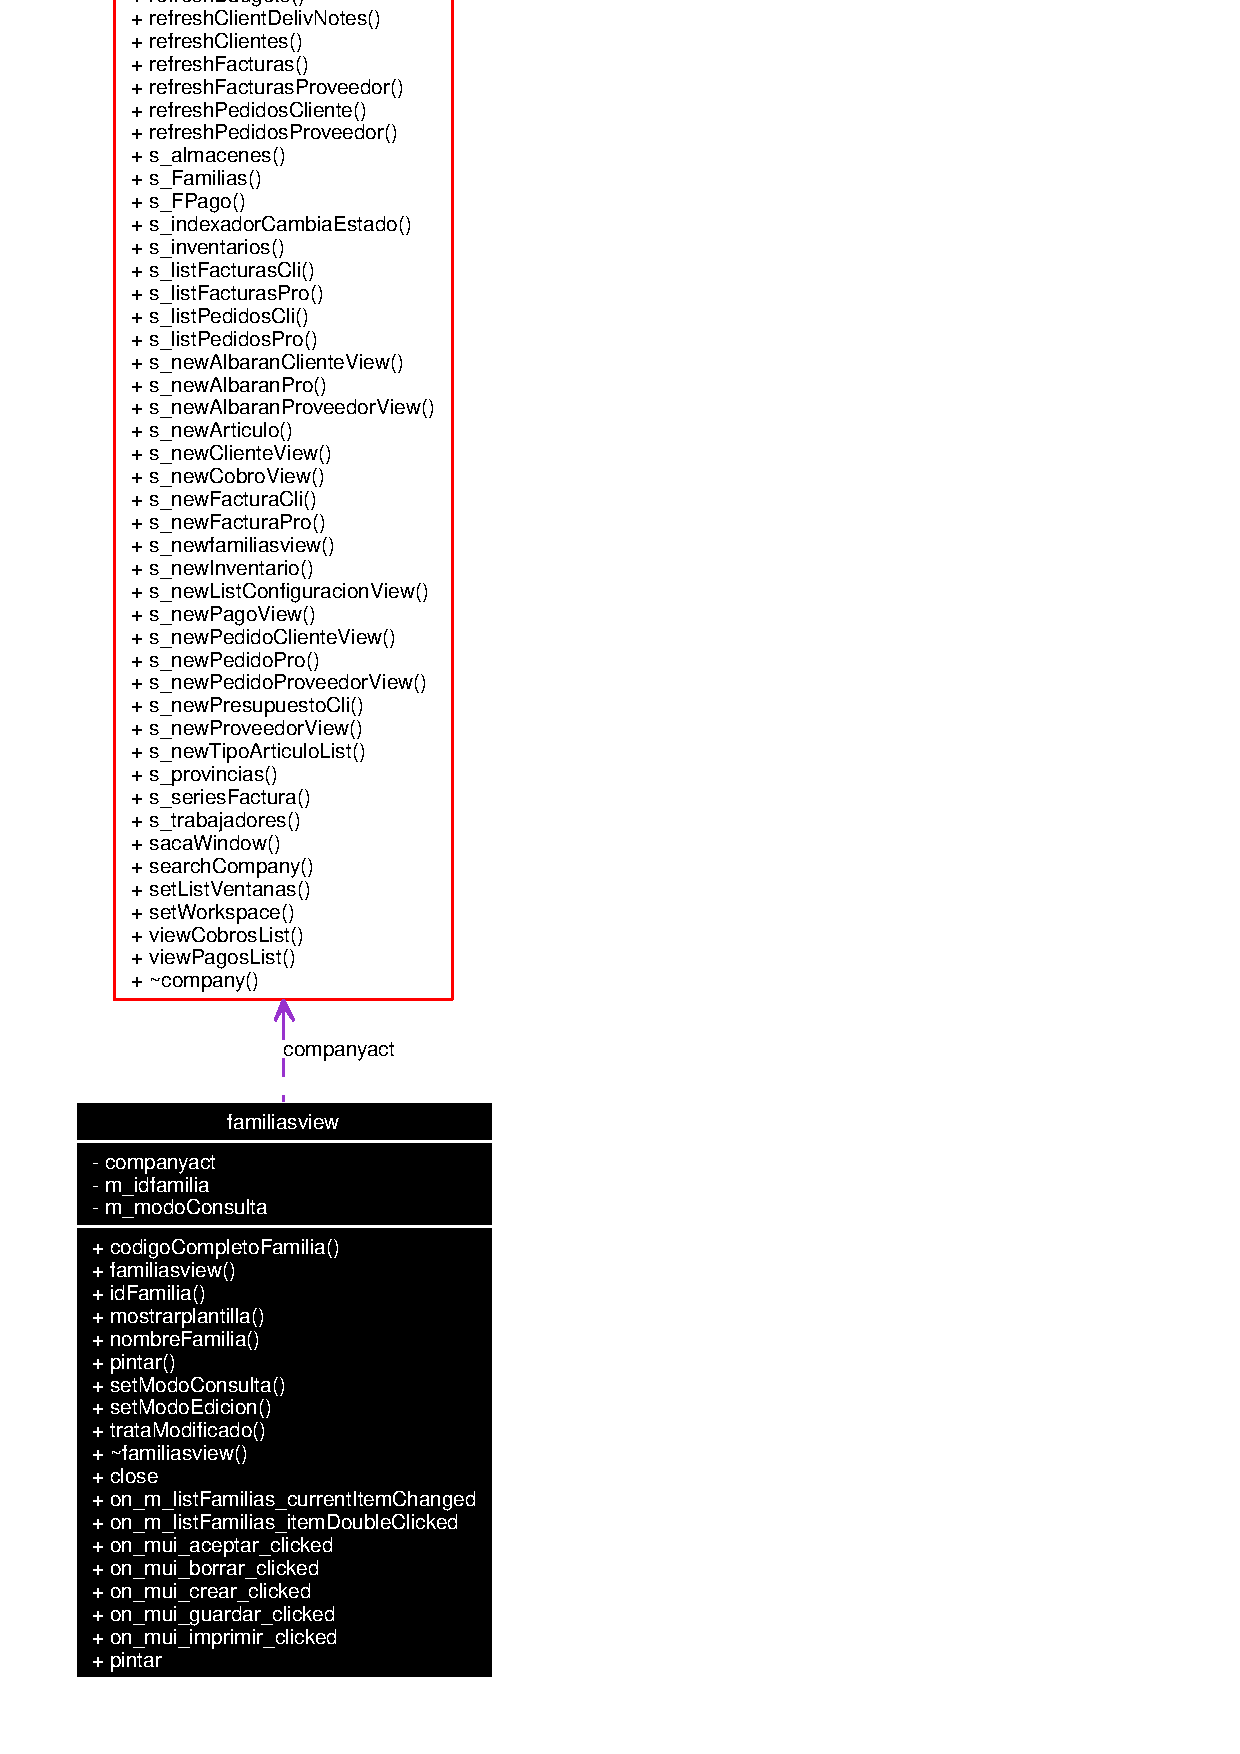
\includegraphics[width=118pt]{classfamiliasview__coll__graph}
\end{center}
\end{figure}
\subsection*{Slots p\'{u}blicos}
\begin{CompactItemize}
\item 
virtual void {\bf close} ()
\item 
virtual void {\bf on\_\-m\_\-list\-Familias\_\-current\-Item\-Changed} (QTree\-Widget\-Item $\ast$current, QTree\-Widget\-Item $\ast$previous)
\item 
virtual void {\bf on\_\-m\_\-list\-Familias\_\-item\-Double\-Clicked} (QTree\-Widget\-Item $\ast$)
\item 
virtual void {\bf on\_\-mui\_\-aceptar\_\-clicked} ()\label{classfamiliasview_i3}

\item 
virtual void {\bf on\_\-mui\_\-borrar\_\-clicked} ()
\item 
virtual void {\bf on\_\-mui\_\-crear\_\-clicked} ()
\item 
virtual void {\bf on\_\-mui\_\-guardar\_\-clicked} ()
\item 
virtual void {\bf on\_\-mui\_\-imprimir\_\-clicked} ()
\item 
virtual void {\bf pintar} ()
\end{CompactItemize}
\subsection*{Se\~{n}ales}
\begin{CompactItemize}
\item 
void {\bf selected} (QString)\label{classfamiliasview_l0}

\end{CompactItemize}
\subsection*{M\'{e}todos p\'{u}blicos}
\begin{CompactItemize}
\item 
QString {\bf codigo\-Completo\-Familia} ()\label{classfamiliasview_a0}

\item 
{\bf familiasview} ({\bf company} $\ast$, QWidget $\ast$parent=0, bool modo\-Consulta=FALSE)\label{classfamiliasview_a1}

\item 
QString {\bf id\-Familia} ()\label{classfamiliasview_a2}

\item 
void {\bf mostrarplantilla} ()
\item 
QString {\bf nombre\-Familia} ()\label{classfamiliasview_a4}

\item 
void {\bf pintar} (QTree\-Widget\-Item $\ast$)\label{classfamiliasview_a5}

\item 
void {\bf set\-Modo\-Consulta} ()\label{classfamiliasview_a6}

\item 
void {\bf set\-Modo\-Edicion} ()\label{classfamiliasview_a7}

\item 
bool {\bf trata\-Modificado} ()
\end{CompactItemize}


\subsection{Descripci\'{o}n detallada}
Muestra y administra la ventana de familias de art\'{\i}culos. 



\subsection{Documentaci\'{o}n de las funciones miembro}
\index{familiasview@{familiasview}!close@{close}}
\index{close@{close}!familiasview@{familiasview}}
\subsubsection{\setlength{\rightskip}{0pt plus 5cm}void familiasview::close ()\hspace{0.3cm}{\tt  [virtual, slot]}}\label{classfamiliasview_i0}


Antes de salir de la ventana debemos hacer la comprobacion de si se ha modificado algo Esta funcion esta dedicada a Francina, Bienvenida al mundo :)) \index{familiasview@{familiasview}!mostrarplantilla@{mostrarplantilla}}
\index{mostrarplantilla@{mostrarplantilla}!familiasview@{familiasview}}
\subsubsection{\setlength{\rightskip}{0pt plus 5cm}void familiasview::mostrarplantilla ()}\label{classfamiliasview_a3}


Comprobamos cual es la cadena inicial. \index{familiasview@{familiasview}!on_m_listFamilias_currentItemChanged@{on\_\-m\_\-listFamilias\_\-currentItemChanged}}
\index{on_m_listFamilias_currentItemChanged@{on\_\-m\_\-listFamilias\_\-currentItemChanged}!familiasview@{familiasview}}
\subsubsection{\setlength{\rightskip}{0pt plus 5cm}void familiasview::on\_\-m\_\-list\-Familias\_\-current\-Item\-Changed (QTree\-Widget\-Item $\ast$ {\em current}, QTree\-Widget\-Item $\ast$ {\em previous})\hspace{0.3cm}{\tt  [virtual, slot]}}\label{classfamiliasview_i1}


Se ha seleccionado un item en la lista. Lo que hacemos es mostar el elemento. Si el anterior ha sido modificado pedimos para actuar en consecuencia. \index{familiasview@{familiasview}!on_m_listFamilias_itemDoubleClicked@{on\_\-m\_\-listFamilias\_\-itemDoubleClicked}}
\index{on_m_listFamilias_itemDoubleClicked@{on\_\-m\_\-listFamilias\_\-itemDoubleClicked}!familiasview@{familiasview}}
\subsubsection{\setlength{\rightskip}{0pt plus 5cm}void familiasview::on\_\-m\_\-list\-Familias\_\-item\-Double\-Clicked (QTree\-Widget\-Item $\ast$ {\em it})\hspace{0.3cm}{\tt  [virtual, slot]}}\label{classfamiliasview_i2}


Se ha seleccionado un item en la lista. Lo que hacemos es mostar el elemento. Si el anterior ha sido modificado pedimos para actuar en consecuencia. \index{familiasview@{familiasview}!on_mui_borrar_clicked@{on\_\-mui\_\-borrar\_\-clicked}}
\index{on_mui_borrar_clicked@{on\_\-mui\_\-borrar\_\-clicked}!familiasview@{familiasview}}
\subsubsection{\setlength{\rightskip}{0pt plus 5cm}void familiasview::on\_\-mui\_\-borrar\_\-clicked ()\hspace{0.3cm}{\tt  [virtual, slot]}}\label{classfamiliasview_i4}


SLOT que responde a la pulsacion del bot\~{A}179n de borrar la familia que se est\~{A}!` editando. Lo que hace es que se hace un update de todos los campos. \index{familiasview@{familiasview}!on_mui_crear_clicked@{on\_\-mui\_\-crear\_\-clicked}}
\index{on_mui_crear_clicked@{on\_\-mui\_\-crear\_\-clicked}!familiasview@{familiasview}}
\subsubsection{\setlength{\rightskip}{0pt plus 5cm}void familiasview::on\_\-mui\_\-crear\_\-clicked ()\hspace{0.3cm}{\tt  [virtual, slot]}}\label{classfamiliasview_i5}


SLOT que responde a la pulsacion del boton de nuevo tipo de IVA Inserta en la tabla de IVAs.

Si se ha modificado el contenido advertimos y guardamos. \index{familiasview@{familiasview}!on_mui_guardar_clicked@{on\_\-mui\_\-guardar\_\-clicked}}
\index{on_mui_guardar_clicked@{on\_\-mui\_\-guardar\_\-clicked}!familiasview@{familiasview}}
\subsubsection{\setlength{\rightskip}{0pt plus 5cm}void familiasview::on\_\-mui\_\-guardar\_\-clicked ()\hspace{0.3cm}{\tt  [virtual, slot]}}\label{classfamiliasview_i6}


SLOT que responde a la pulsacion del boton de guardar el tipo de IVA que se esta editando. Lo que hace es que se hace un update de todos los campos. \index{familiasview@{familiasview}!on_mui_imprimir_clicked@{on\_\-mui\_\-imprimir\_\-clicked}}
\index{on_mui_imprimir_clicked@{on\_\-mui\_\-imprimir\_\-clicked}!familiasview@{familiasview}}
\subsubsection{\setlength{\rightskip}{0pt plus 5cm}void familiasview::on\_\-mui\_\-imprimir\_\-clicked ()\hspace{0.3cm}{\tt  [virtual, slot]}}\label{classfamiliasview_i7}


Copiamos el archivo.

Copiamos el logo.

Linea de totales del presupuesto. \index{familiasview@{familiasview}!pintar@{pintar}}
\index{pintar@{pintar}!familiasview@{familiasview}}
\subsubsection{\setlength{\rightskip}{0pt plus 5cm}void familiasview::pintar ()\hspace{0.3cm}{\tt  [virtual, slot]}}\label{classfamiliasview_i8}


Vaciamos el arbol.

Comprobamos cual es la cadena inicial. \index{familiasview@{familiasview}!trataModificado@{trataModificado}}
\index{trataModificado@{trataModificado}!familiasview@{familiasview}}
\subsubsection{\setlength{\rightskip}{0pt plus 5cm}bool familiasview::trata\-Modificado ()}\label{classfamiliasview_a8}


Si se ha modificado el contenido advertimos y guardamos. 

La documentaci\'{o}n para esta clase fu\'{e} generada a partir de los siguientes archivos:\begin{CompactItemize}
\item 
familiasview.h\item 
familiasview.cpp\end{CompactItemize}
